%%%%%%%%%%%%%%%%%%%%%%%%%%%%%%%%%%%%%%%%%%%%%%%%%%%%%%
\section{The Standard Model}\label{secSM:ch1}

%"Theorists can be wrong; only nature is always right" - David Gross
"Fortunately, nature is as generous with its problems as Nobel with his fortune. The more we know, the more aware we are of what we know not."- David Gross \newline

The Standard Model, SM, of particle physics constitues humanity's latest attempt at describing our universe in a calculable way. The basic premise being, the entire universe is compised solely of; 6 types of quark and 6 types of lepton, which comprise matter, and the guage bosons, which mediate the 3 (this theory does not yet encompass gravitaion) fundamental forces; The strong and weak nuclear interactions and electromagnetism. 


Various attempts have been made to unify the fundamental forces under one theory, thusfar the electromagnetic and weak interactions have been united by electro-weak theory. 

The Standard electroweak model can be described $SU(2) x U(1)$ mathematically.

The  $SU(2) x U(1)$ guage group is a convolution ( $<- $That is not the right word...) of the special unitary symmetry group $SU(2)$ describing 3 mixed massive vector bosons, $W_{-}$ $W_{+}$ $Z_0$, carriers of the weak nuclear force and the unitary gauge group $U(1)$ , describing the lonely massless chargeless photon, of the electromagnetic interaction.

The standard model of the strong interaction is known as quatum chromodynamics, QCD, described by the special unitary group $(SU(3)_f)$, where the  flavours of quark are the physical manifestation of the symmetry group. This force is mediated by the 8 massless gluons which carry color charge, making QCD more complicated mathematically than QED.

The SM also contains a Higgs boson, an excitation of a scalar Higg's field, which gives rise to spantaneous symmetry breaking of the electroweak theory, providing the particles with mass, but I won't get into that. 

The quarks and leptons are arranged in generations according to their relative masses, as shown in Figure \ref{fig:SM}. The table also shows the spins of the particles, the leptons and quarks have half-integer spin, fermions, that obey the fermi exclusion principle, conversely the bosons have half integer spin and therefore obey bose-einstein statitics. Through the SM we interpret the observed hadronic particles, mesons ( baryons ) , as 2 quark (3 quark) bound states. The existence of spin $\frac{3}{2}$ baryons, which are symmetric bound states in space, spin and flavour and the need to obey Fermi-Dirac statistics, by maintaining total assymmetry of the wavefunction,implies there is another degree of freedom, called color, so that each quark is either red, green or blue. Granted only color singlet, containing either all 3 or 1 and it's anti color, states exist. Furthermore there exists a property of asymptotic freedom where the QCD coupling between quarks and gluons increases as they asymptotically approach one another. There exists a wealth of experiemental data to support the concept of asymptotic freedom despite the fact that rigorous mathematical proof of the exlusion of free quark and gluon states has yet to be acheived.

Assymptotic freedom is a useful property as it allows for perturbative calculations of QCD observables, this is discussed in section XXX.

% Symmetris imply conserved quantities, Neuther's Theorem

 Nuclei in ordinary matter are composed solely of $1^{st}$ generation particles, up and down quarks, bound by gluons. Neutral atoms contain an equal number of protons (composed of 2 up quarks and a down quark) and electrons, $1^{st}$ generation leptons. The main distinction between leptons and quarks, both fermions (particles of $\frac{1}{2}$ integer spin), being that leptons do not experience the color interaction $(SU(3)_f)$ like their quark friends. In each generation there is a quark with charge $Q = + \frac{2}{3}$ (up, charm, top) and another of charge $Q = - \frac{1}{3}$ (down, strange, bottom).



\begin{figure}[htb]
\centering
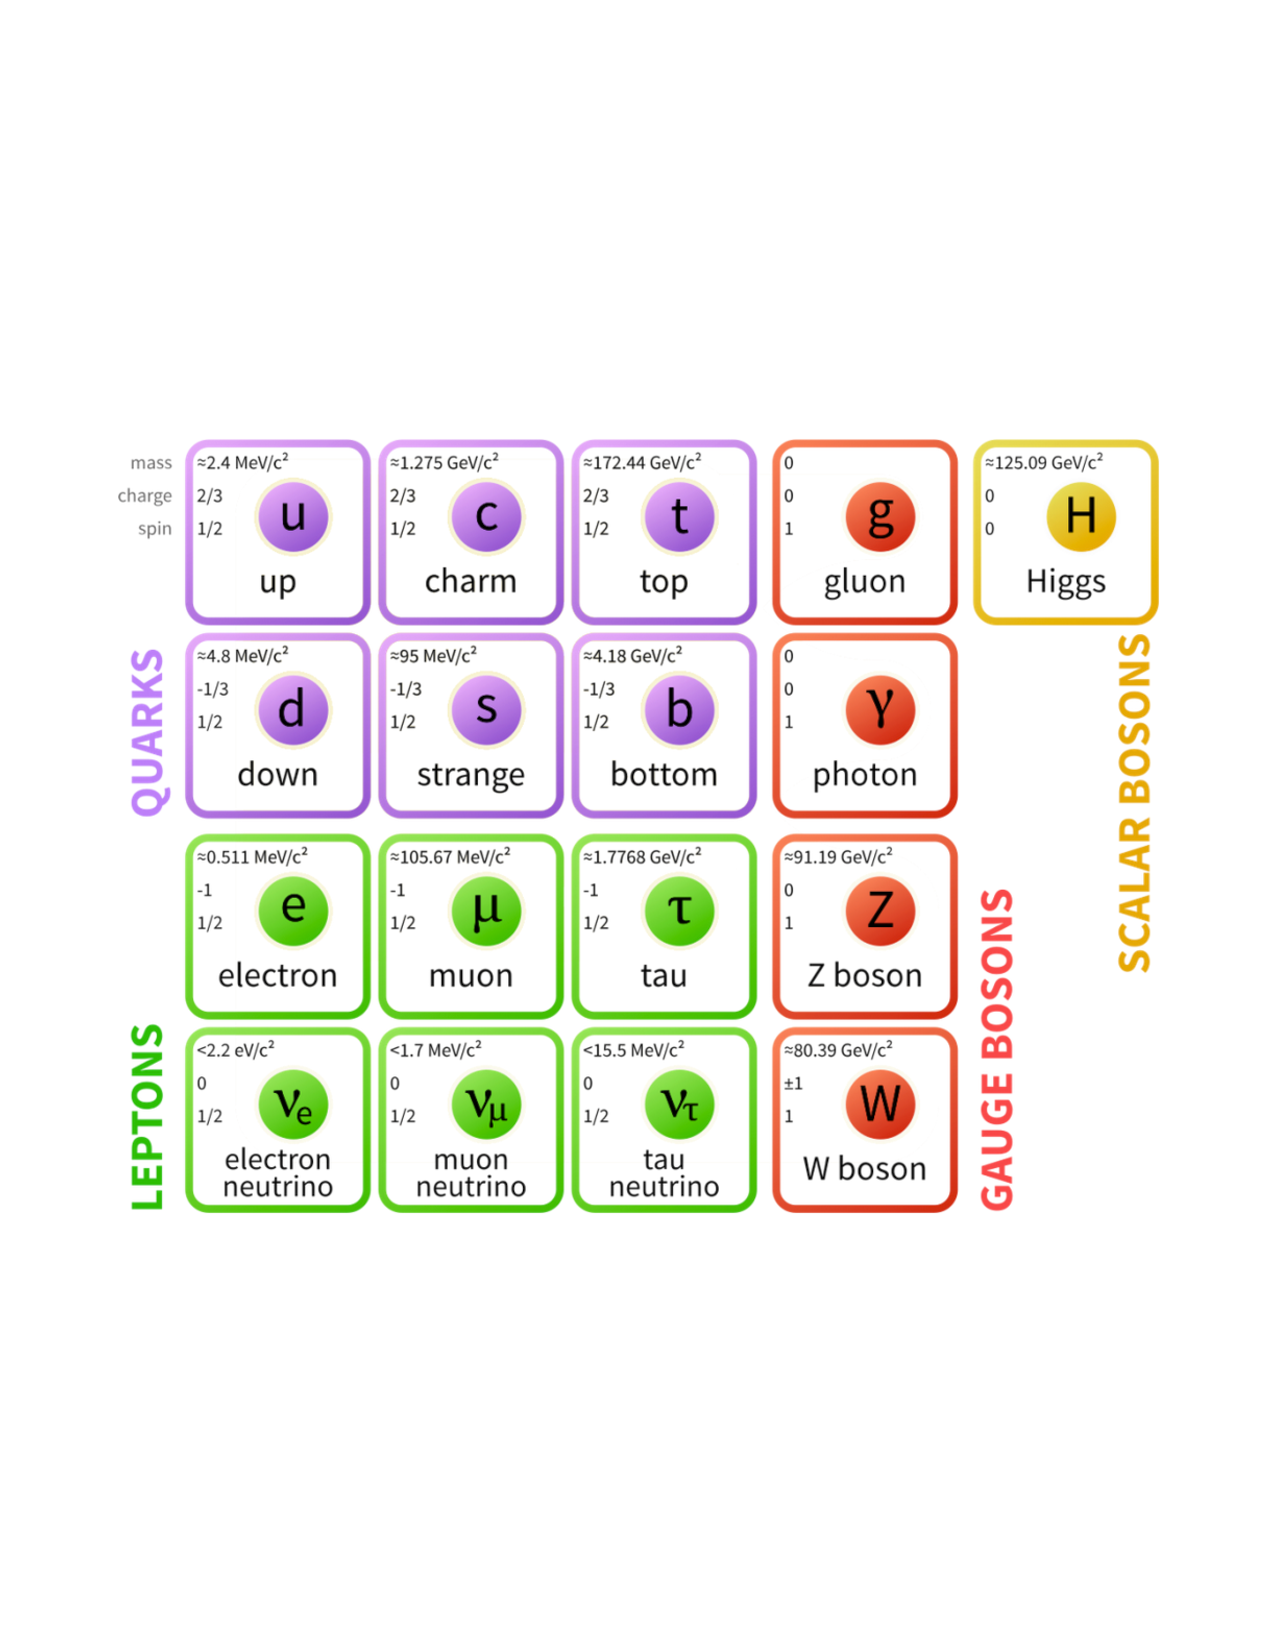
\includegraphics[width=1.0\textwidth]{smdiagram.pdf}
\caption{Fundamental particles of the Standard Model~\cite{modellinginvisible}.}
\label{fig:SM}
\end{figure}






\subsection{Quantum Chromodynamics}\label{secSM:ch1}


For the purpose of this thesis, in order to emphasize the relevance to jet substructure measurements, I will discuss the theory of Quantum Chromodynamics from a kinematic (<- better word?) rather than Lagrangian perspective. This is useful as the jet studies presented here help probe QCD in the soft and collinear limits. 
% https://arxiv.org/pdf/1709.06195.pdf CITE THIS LECTURE
Jets are formed by the hadronization of quarks and gluons. In this thesis I present a measurement of a light quark enriched jet samples. Consider the simplest process that could produce a quark initiated jet, a quark of energy $E_q$  emitting a gluon of energy $E_g$. The probability that this will occur is a function of the gluon's energy fraction, $z$, and the emission angle , $\theta$.\newline


$z = \frac{E_g}{E_q + E_g}$\newline

$1 - cos \theta = \frac{m^2}{2 E_q E_g}$\newline

Then the probability of gluon emission from the quark is :


$P_q(z,cos \theta) dz d cos \theta = \frac{\alpha_s C_F}{\pi}  \frac{dz}{z} \frac{dcos \theta}{1 - cos \theta}  $\newline

It is useful to assume the small angle approximation, $\theta << 1$, giving:\newline


$P_q(z,\theta^2) dz d \theta^2 = \frac{\alpha_s C_F}{\pi}  \frac{dz}{z} \frac{d \theta^2}{ \theta^2}  $\newline

Notice that the probability of emission diverges for very soft (small z) or very collinear (small $\theta$) gluons.

It is elucidating to rewite the probability in terms of inverse logarithms in the and intruduce the "Lund Diagram" in order to visualize the uniform distribution of soft and collinear gluons in the $log \frac{1}{ \theta^2} , log\frac{1}{z} $ space.



$P_q(z,\theta^2) dz d \theta^2 = \frac{\alpha_s C_F}{\pi} d( log\frac{1}{z}  ) d(log \frac{1}{ \theta^2})  $\newline

Jets can also be initiated by gluons and this probability is incredibly similar :


$P_q(z,\theta^2) dz d \theta^2 = \frac{\alpha_s C_A}{\pi} d( log\frac{1}{z}  ) d(log \frac{1}{ \theta^2})  $\newline


This similarity allows us to interpret the variations in quark enriched and gluon enriched jet samples in terms of the $C_F$ and $C_A$, in $SU(3)$ ,   $C_F = \frac{4}{3}$ and $C_A=3$.


